
%\RequirePackage{pdf15}

\documentclass{beamer}

\usepackage[utf8]{inputenc}

\usepackage{mystyle}

\usepackage{tikz}
\usepackage{pgfplots}
\usepackage{subcaption}

\usepackage{natbib}
\bibliographystyle{apalike}
%\usepackage[style=authortitle,backend=biber]{biblatex}
%\addbibresource{anthology.bib}
%\addbibresource{emnlp2020.bib}
\renewcommand{\footnotesize}{\scriptsize}

\usepackage{tikz-dependency}
\usetikzlibrary{shapes.arrows, positioning, fit, bayesnet,
    arrows,backgrounds,patterns,matrix,calc,shadows,plotmarks,
    shapes,positioning,automata,positioning,spy,scopes,chains,decorations,decorations.pathreplacing}

\newcommand{\FancyUpArrow}{
\begin{tikzpicture}[baseline=-0.3em]
\node[single arrow,draw,rotate=90,single arrow head extend=0.2em,inner
ysep=0.2em,transform shape,line width=0.05em,top color=green,bottom color=green!50!black] (X){};
\end{tikzpicture}}
\newcommand{\FancyDownArrow}{
\begin{tikzpicture}[baseline=-0.3em]
\node[single arrow,draw,rotate=-90,single arrow head extend=0.2em,inner
ysep=0.2em,transform shape,line width=0.05em,top color=red,bottom color=red!50!black] (X){};
\end{tikzpicture}}

\AtBeginSection[]{
  \begin{frame}
  \vfill
  \centering
  \begin{beamercolorbox}[sep=8pt,center,shadow=true,rounded=true]{title}
    \usebeamerfont{title}\insertsectionhead\par%
  \end{beamercolorbox}
  \vfill
  \end{frame}
}

% quotes
\usepackage[style=british]{csquotes}

\def\signed #1{{\leavevmode\unskip\nobreak\hfil\penalty50\hskip1em
  \hbox{}\nobreak\hfill #1%
  \parfillskip=0pt \finalhyphendemerits=0 \endgraf}}

\newsavebox\mybox
\newenvironment{aquote}[1]
  {\savebox\mybox{#1}\begin{quote}\openautoquote\hspace*{-.7ex}}
  {\unskip\closeautoquote\vspace*{1mm}\signed{\usebox\mybox}\end{quote}}

%Information to be included in the title page:
\title{Word Games}
\author{J Chiu}

\setbeamertemplate{navigation symbols}{} 
\setbeamertemplate{footline}[frame number]

\begin{document}

\begin{frame}[plain]
\titlepage
\end{frame}

\begin{frame}
\frametitle{Coordination and dialogue}
\begin{columns}
\begin{column}{0.5\textwidth}
\begin{itemize}
\item Coordination
    \begin{itemize}
    \item I
    \end{itemize}
\item Interactive reference games
    \begin{itemize}
    \item Isolates ambiguity resolution
    \end{itemize}
\end{itemize}
\end{column}
\begin{column}{0.5\textwidth}
    \centering
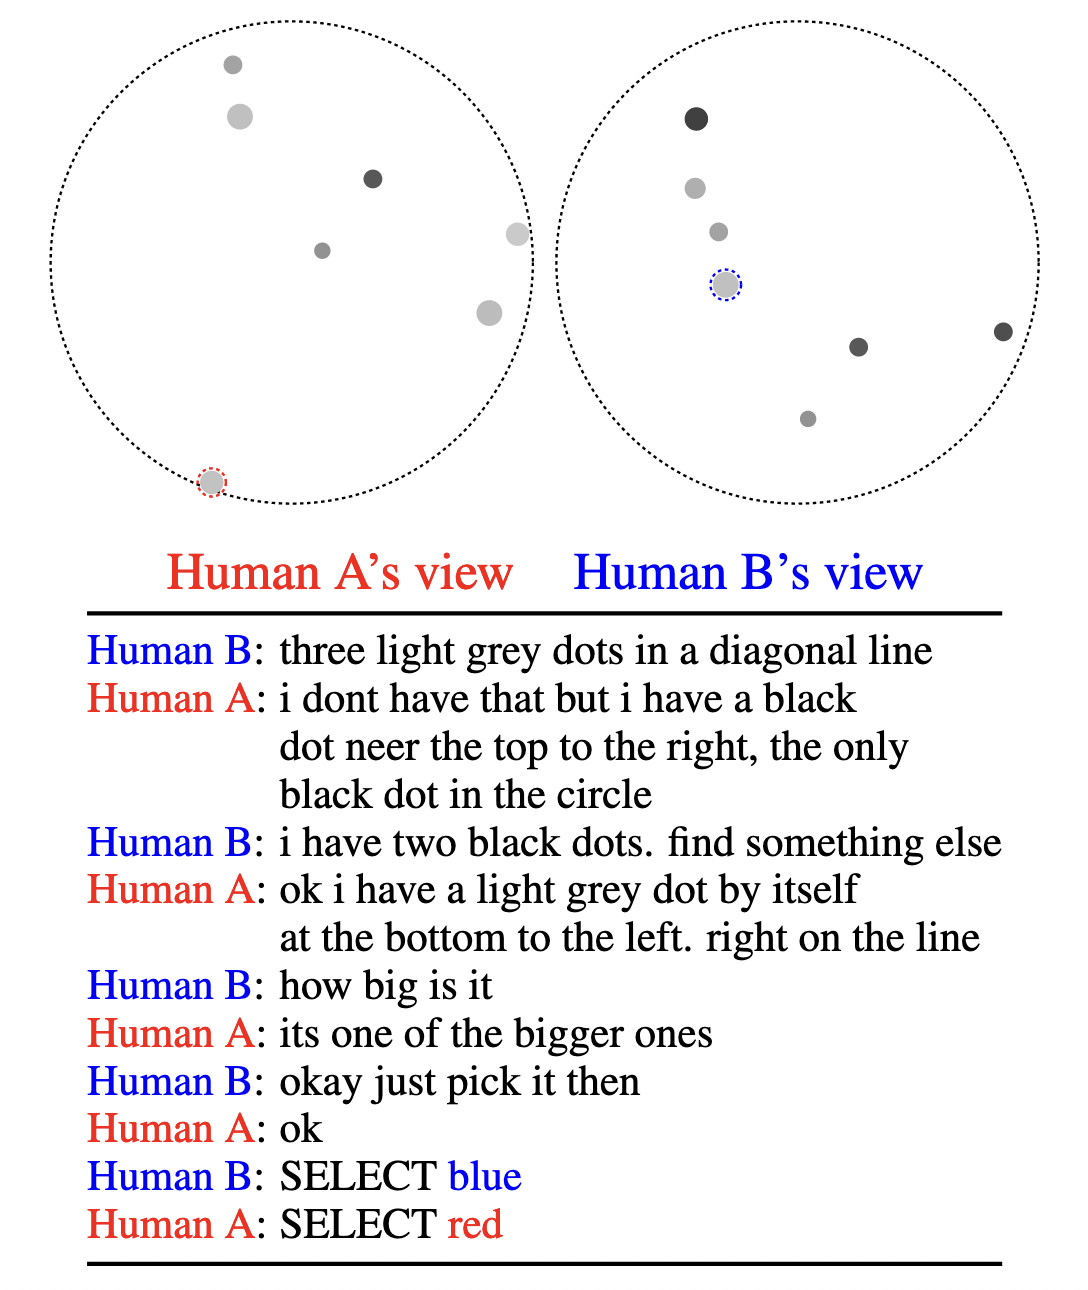
\includegraphics[width=2in]{img/oc.png}
\end{column}
\end{columns}
\end{frame}

\begin{frame}
\frametitle{Games}

\begin{columns}
\begin{column}{0.5\textwidth}
\centering
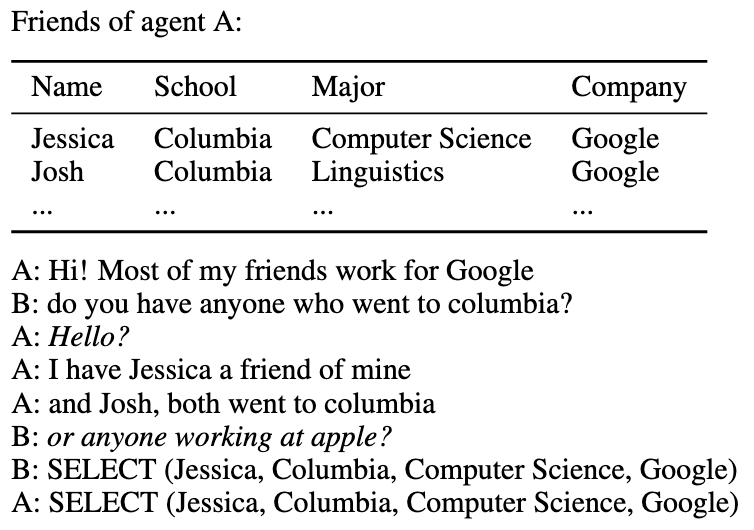
\includegraphics[width=2in]{img/mf.png}
\end{column}
\begin{column}{0.5\textwidth}
\centering
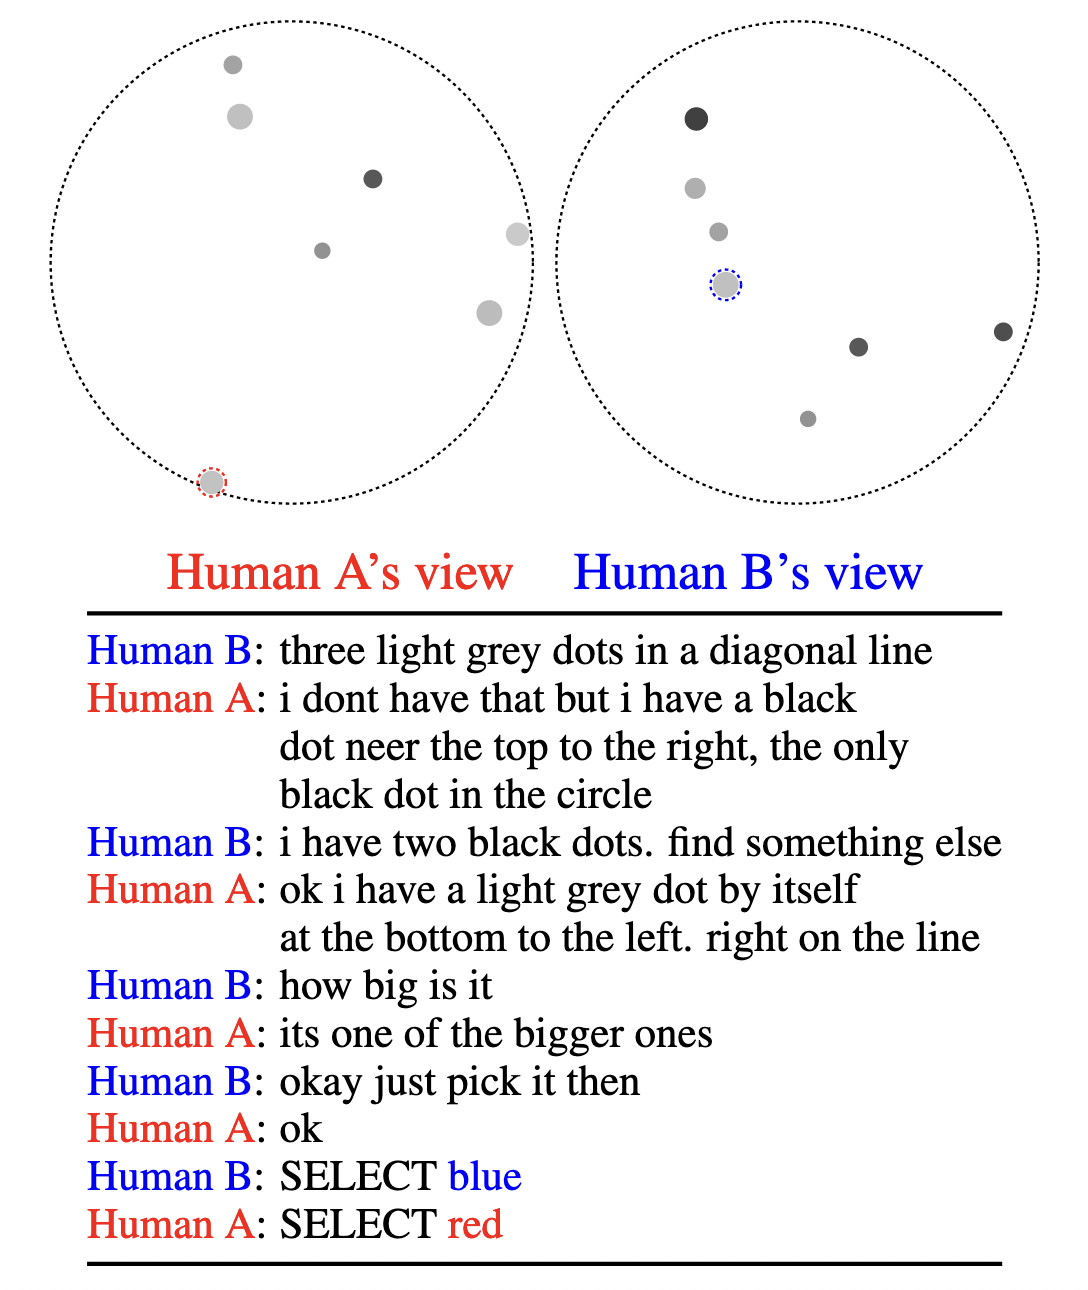
\includegraphics[width=2in]{img/oc.png}
\end{column}
\end{columns}

\vspace{2em}
\centering
Mutual Friends and OneCommon
\end{frame}

\begin{frame}
\frametitle{Current Approaches}
\begin{itemize}
\item Neural encoder-decoder
    \begin{itemize}
    \item Encode past interactions with a neural net
    \item Generate what to say with a neural net
    \item Less brittle for language, brittle strategy
    \end{itemize}
\item Rule-based
    \begin{itemize}
    \item Encode past interactions in a table
    \item Use rules for what to say next
    \item Nonparametric lookup of utterances
    \item Less brittle strategy, brittle language
    \end{itemize}
\item Let's see some examples of brittleness
    from these two domains
\end{itemize}
\end{frame}

\begin{frame}
\frametitle{Issue 1: Poor strategies}
\begin{itemize}
\item 
\end{itemize}
\end{frame}

\begin{frame}
\frametitle{Issue 2: }
\begin{itemize}
\item Asdf
\end{itemize}
\end{frame}

\begin{frame}
\frametitle{A dialogue turn}
\begin{itemize}
\item Engaging in dialogue requires
    \begin{itemize}
    \item Inference: What information do I currently have?
    \item Planning: What should I say (and how)?
    \end{itemize}
\item Formulate as model-based optimization
    \begin{itemize}
    \item Plan what to say through a simple model of our partner
    \item Model of partner conditions on past information
    \end{itemize}
\end{itemize}
\end{frame}

\begin{frame}
\frametitle{Problem setup}
\begin{itemize}
\item Sequential decision process
\item 
\end{itemize}
\end{frame}

\begin{frame}
\frametitle{Reference Dialogue Games}
\begin{itemize}
\item Simplest form of collaborative task-oriented dialogue
\item Convey a referrent to your dialogue partner
    \begin{itemize}
    \item Ex: Jointly selecting a star
    \end{itemize}
\item Successful joint attention = task success

\item Simplest form: Information gathering via discriminative questions
    \begin{itemize}
    \item Can also include coordination (OC, MutualFriends) focus on this
    \item Or even navigation (Cards)
    \end{itemize}

\end{itemize}
\end{frame}

\begin{frame}
\frametitle{Solving Reference Games}
\begin{itemize}
\item Multiple agents with equal capabilities
    \begin{itemize}
    \item Pro: More efficient task completion
    \item Con: May be more difficult to reason about other agents' belief states
        (`agent uncertainty')
    \end{itemize}
\item Natural language dialogue
    \begin{itemize}
    \item Pro: Great for interfacing with non-experts
    \item Con: Extremely large search space when planning
    \end{itemize}
\item Planning in a structured action / observation space
    \begin{itemize}
    \item Pro: Computationally efficient planning
    \item Con: Must convert to and from language, leading to `sensor uncertainty'
    \end{itemize}
\end{itemize}
\end{frame}

\begin{frame}
\frametitle{Research question}
\begin{itemize}
\item How can we achieve joint attention, a necessary first step towards collaboration?
\item Hypothesis: We can solve joint attention with efficient and accurate planning
    \begin{itemize}
    \item Past work planning directly in language is inefficient and inaccurate
    \item Reference games admit a natural structured action / observation space
    \end{itemize}
\item Challenge: Planning is computationally difficult in multi-agent systems
    \begin{itemize}
    \item Large number of belief states
    \item Difficult to calibrate sensor uncertainty with language
    \end{itemize}
\end{itemize}
\end{frame}

\begin{frame}
\frametitle{OneCommon}
Collaborative reference game where the goal is to find one dot
both players have in common,
given different but overlapping views
\begin{center}
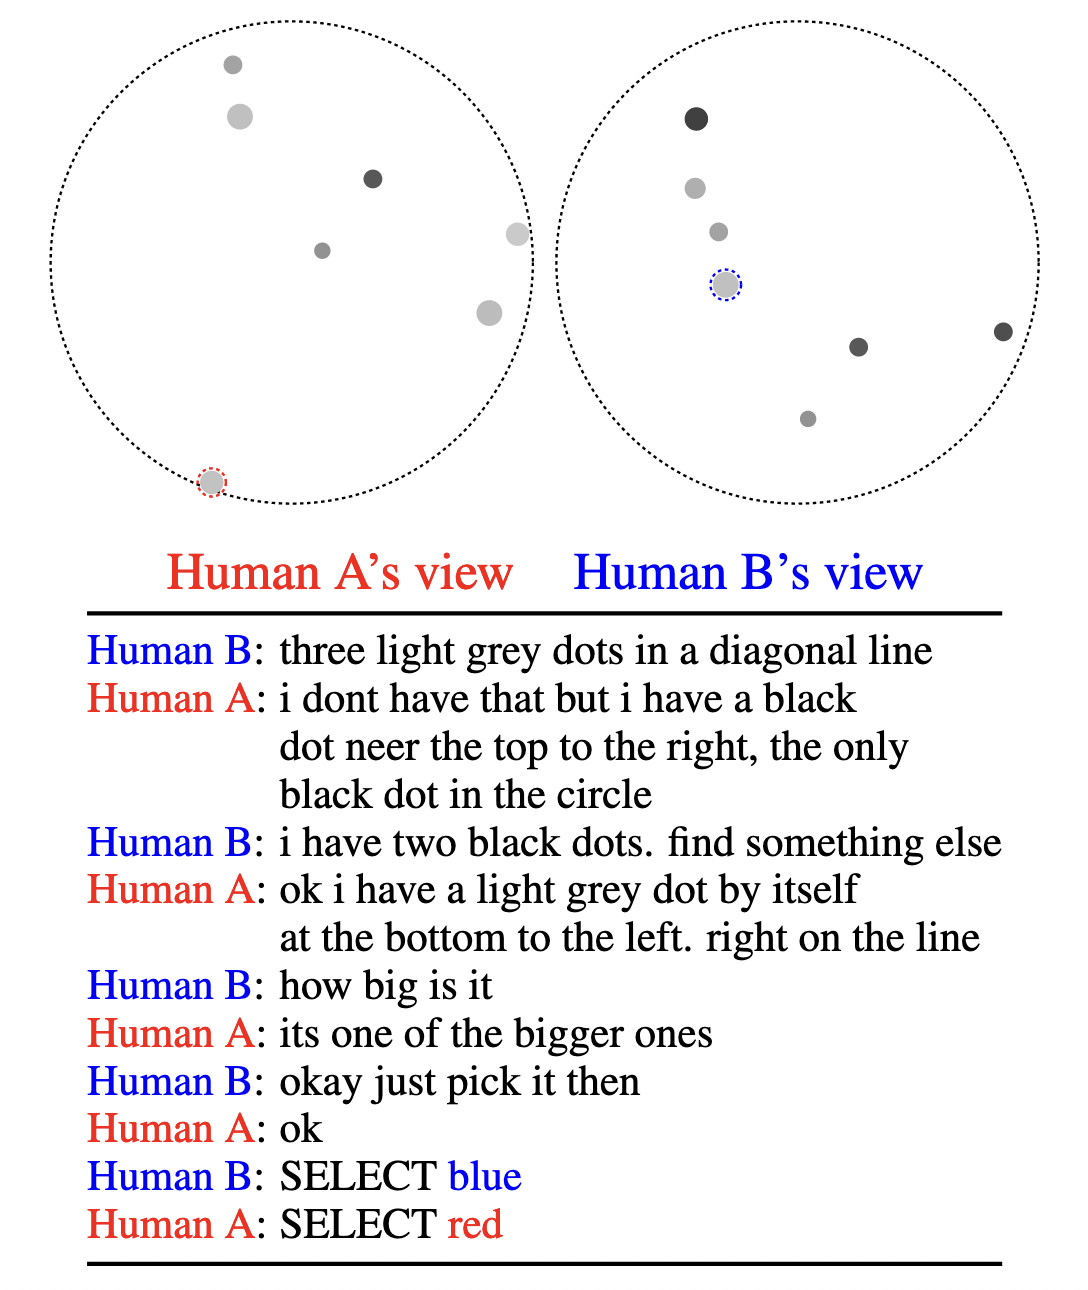
\includegraphics[width=2in]{img/oc.png}
\end{center}
\end{frame}

\begin{frame}
\frametitle{Method}
\begin{itemize}
\item Separate language (sensors) from planning
\item Formalize problem as a decentralized POMDP
    \begin{itemize}
    \item Players are performing hypothesis testing together
    \end{itemize}
\item Sources of uncertainty
    \begin{itemize}
    \item Language input (sensors)
    \item Language output (generation errors)
    \item Other agents
    \end{itemize}
\item Focus on uncertainty induced by other agents
    \begin{itemize}
    \item Is modeling other agents' beliefs necessary?
    \end{itemize}
\end{itemize}
\end{frame}

\begin{frame}
\frametitle{Research Questions Summary}
\begin{itemize}
\item Goal: Solve joint attention
\item Question: Can we solve joint attention by utilizing structure to improve the
    efficiency and accuracy of planning?
\item Additionally: When is modeling other agents' beliefs necessary?
\end{itemize}
\end{frame}

\begin{frame}
\frametitle{Current Status}
\begin{itemize}
\item POMDP formulation as best-arm identification (Simplification, ignores dec)
    \begin{itemize}
    \item Symmetric actions and observations for both partners (Good!)
    \item Actions and observations are structured
    \item Include extra information as a `free turn' in POMDP
    \item Ignores partner belief
    \end{itemize}
\item Planning ignores structure (inefficient, but ok for now)
\item Solves small state space (each can see 3 dots with 1 shared) and
    all dots unique / easily identified
\item Next step: See if partner belief modeling is necessary
    when dots are not as easily identified
\end{itemize}
\end{frame}

\begin{frame}
\frametitle{Deprecated below}
See belief writeup for more up to date stuff
\end{frame}

\begin{frame}
\frametitle{Related Work}
\begin{itemize}
\item Lots of work decoupling actions from language (to avoid catastrophic forgetting)
\item Aligning text to (continuous) actions \citep{latentactions}
\item Modern implementation of Cards \citep{cards}?
    \begin{itemize}
    \item Is the Dec necessary? (How different is I'm sure from they're sure) 
    \item Is the PO part important, i.e. can we use certainty equivalence?
        (low risk, how often do edge cases occur?)
    \item Amortized inference, better approximation algorithms / search?
    \end{itemize}
\end{itemize}
\end{frame}

\begin{frame}
\frametitle{OneCommon: Properties}
\begin{itemize}
\item Action space: Can be reduced to predicates over dots and boolean response
    to partner predicates
\item Observations: Observations are symmetric with action space
\item Agents: Only one other agent, which we can assume is similar
\item Strategy: Mostly common to other reference games
\end{itemize}
\end{frame}

\begin{frame}
\frametitle{Simplified OneCommon}
We can solve the following POMDP almost exactly with value iteration
\begin{itemize}
\item Small horizon $T=5$
\item State: Beta distribution for each dot.
    Gives prior over our partner having a dot.
    Combine independent Beta parameters into Dirichlet for selection.
\item Actions: We communicate directly in a single predicate over our dots
    ($2^{D}$ different predicates)
\item Observations: Partner can only respond to predicate noiselessly
\end{itemize}
We can almost solve the Bellman equation
\begin{itemize}
\item Convert to and MDP over belief state
\item Reduce belief state to sufficient statistics of positive response counts for each dot
    (of size $T^D$)
\item Transitions limited because we can only add 1 or 0 to counts
\item Major issue is max over actions
\end{itemize}
\end{frame}

\begin{frame}
\frametitle{Next Steps}
Shorter term
\begin{itemize}
\item Align language to actions (predicates over our dots)
\item Add noise to feedback (did they understand our action/predicate?)
\end{itemize}
Longer term
\begin{itemize}
\item Extend response from boolean (they can offer more information, ask questions)
\item Approximate methods for larger state space (MCTS used in prior work with actions = language),
    i.e. MutualFriends
\end{itemize}
Longerer term
\begin{itemize}
\item Dec-POMDP
\end{itemize}
\end{frame}

\begin{frame}
\frametitle{VERY OLD SLIDES. DO NOT CONTINUE}
\end{frame}

\begin{frame}
\frametitle{Motivation: Why OneCommon}
\begin{itemize}
\item OneCommon is all about referring expressions (resolving / generating)
\item Focus on improving reference resolver, text has more noise
\item Improve generation using reference resolver
\item Goal: Reduce as much learning as possible to reference resolver
\item Impact: Need to carry over to referring expressions in other settings
\end{itemize}
\end{frame}

\begin{frame}
\frametitle{Current OneCommon Performance}
\begin{itemize}
\item How can we improve the reference resolver?
    \begin{itemize}
    \item Best model gets 93\% accuracy 78\% exact match
    \item Human is 96\% accuracy 87\% exact match
    \item Does fine-tuning pretrained models improve accuracy of reference resolver?
    \item How can we close the gap?
    \end{itemize}
\item Would a better reference resolver result in a better selection model?
    \begin{itemize}
    \item Yes, training on true refs gives 99\% accuracy selection model
    \item Best model currently at 83\%, humans at 91\%
    \end{itemize}
\item Does fine-tuning pretrained models improve round-trip of reference generator?
    \begin{itemize}
    \item Generation second priority
    \item Likely over-fitting
    \end{itemize}
\end{itemize}
\end{frame}

\begin{frame}
\frametitle{Current Models for RE}
\begin{itemize}
\item Fried 2021
    \begin{itemize}
    \item Conditions on utterances and marginal dot features
    \item Neural referent memory (updates dots on reference)
    \end{itemize}
\item Udagawa 2021
    \begin{itemize}
    \item Conditions on utterances and marginal dot features (input structure via
        relational networks)
    \end{itemize}
\end{itemize}
\end{frame}

\begin{frame}
\frametitle{Improving RE}
\begin{itemize}
    \item Resolve multiple dots
        \begin{itemize}
        \item Use number prediction to select explicit arity potentials
        \item Not enough data? Gather more data with more ambiguity, i.e. dots
            all have the same size and color? Would this transfer (motivation)?
        \end{itemize}
    \item Architectures that are more biased towards composition
        \begin{itemize}
        \item DIORA
        \item Transformers? (possibly with attention constraints)
        \end{itemize}
    \item Reason explicitly about past references
        \begin{itemize}
        \item Belief state / checklist
        \item Pragmatic inference via mutual exclusivity
            (check if anything is referenced multiple times)
        \end{itemize}
    \item Coreference
        \begin{itemize}
        \item Unfamiliar, need further research
        \item How often does this happen?
        \end{itemize}
   \item Dialogue acts
        \begin{itemize}
        \item Pragmatics of resolution vary based on dialogue act
        \item Confirmation repeats vs new references
        \item How to collect data for this?
        \end{itemize}
\end{itemize}
\end{frame}

\begin{frame}
\frametitle{Generalization / Transfer to Other Tasks}
\begin{itemize}
\item Low-resource datasets that need more structure / bias
\item Context is useful for understanding
    \begin{itemize}
    \item 
    \end{itemize}
\item Understanding is useful for generation
\end{itemize}
\end{frame}

\begin{frame}
\frametitle{3 Challenges}
\begin{itemize}
\item Modular models
    \begin{itemize}
    \item Dialogue model = local meaning representation -
        belief state - dialog act - utterance generation
    \item Various works supervise particular parts
        then leave others to be implicitly learned through
        neural nets
    \item Results in very task-specific architectures
    \item Can we break down tasks to allow for
        more component sharing across different tasks, as well as
        semi-supervised learning?
    \end{itemize}
\item Less complicated meaning representations
    \begin{itemize}
    \item Meaning representations vary in granularity
    \item Can we learn a minimal task-specific subset of a meaning
        representation formalism?
    \end{itemize}
\item Adapting to partners
    \begin{itemize}
    \item Partner model allows forward modeling, learned over
        a multiple round game or repeated games
    \item Adapt opaque neural model or hierarchical bayesian model?
    \end{itemize}
\item Better reference resolution / referring expression models?
    \begin{itemize}
    \item Dialogue games are often data scarce and out of domain
    \item Can we use models that are more sensitive / with stronger
        biases?
    \end{itemize}
\end{itemize}
\end{frame}

\begin{frame}
\frametitle{Natural Language Interaction}
\begin{itemize}
\item Interaction (through language) is important 
    \begin{itemize}
    \item Cannot fully automate every task,
        i.e. task-oriented or information seeking dialogues
        require human input
    \item Must handle diverse non-expert human input,
        although input may map to a low-dimensional manifold
    \item High levels of ambiguity must be resolved via interaction
    \end{itemize}
\item Interaction (through language) is hard 
    \begin{itemize}
    \item Human input is expensive, so supervision is limited
    \item In order to make certain problem aspects tractable,
        must make sacrifices in other areas
        (toy domain = out of distribution for pretrained models)
    \end{itemize}
\item What are the main challenges in interaction,
    and what are the tradeoffs of different approaches?
\end{itemize}
\end{frame}

\begin{frame}
\frametitle{Types of Dialogue Games}
\begin{itemize}

\item Task-oriented: Wizard of Oz (WoZ)
    \begin{itemize}
    \item \citet{tseng2019semisupdialogue}: Wizard obtains
        task from human then executes it.
    \end{itemize}
\item Deliberation / reference / signal
    \begin{itemize}
    \item \citet{udagawa2019oc}: Visual reference game
        with latent translated views.
        Each player gets a different petri dish view
        of the same underlying game board, and players must
        select the same object on the board.
    \end{itemize}
\item Information seeking / inquiry
    \begin{itemize}
    \item \citet{yu2019questions}: WoZ-style answer providing
        where asker does not know exact question.
        Latent true question (to all), WoZ must answer
    \end{itemize}
\item Persuasion / negotiation
    \begin{itemize}
    \item \citet{lewis2017dnd}: Negotiation over an observed
        set of item with latent utilities for each agent.
    \end{itemize}
\end{itemize}
\end{frame}

\begin{frame}
\frametitle{Types of Dialogue Games}
In all cases, the game can be (indirectly) solved by resolving a latent variable

\begin{itemize}
\item When is this tractable, and why do no new methods do this?
\item New (ie basically all) methods rely on supervision
\item If they do not, it is because the game has a trivial solution
\end{itemize}
\end{frame}

\begin{frame}
\frametitle{Talk with Nori}
\begin{itemize}
\item Planning doesnt really exist in most dialogue games,
    the games are too simple
\item Referring expressions in OneCommon can be outliers in terms of complexity.
    Complexity in real world image+text data comes from large noun classes
    and relatively simple phrases.
    Still seems like an interesting testbed though,
    and maybe there is an argument for OneCommon,
    despite its artificial difficulty (maybe people like talking about stars?).
\item Latent variable models for adaptation still seem interesting,
    should read Hawkins' work.
\end{itemize}
\end{frame}

\begin{frame}
\frametitle{Types of Dialogue Games: Latent goals and strategy}
What are the latent variables in each type?
\begin{itemize}
\item Task-oriented
    \begin{itemize}
    \item Latent task slots
    \end{itemize}
\item Deliberation / reference / signal
    \begin{itemize}
    \item Varies per game
    \end{itemize}
\item Information seeking / inquiry
    \begin{itemize}
    \item Infer true question, find answer
    \end{itemize}
\item Persuasion / negotiation
    \begin{itemize}
    \item Infer utilities, exploit
    \end{itemize}
\end{itemize}
\end{frame}

\begin{frame}
\frametitle{Types of Dialogue Games: Latent goals and strategy}
\begin{itemize}
\item Tasks must be interesting enough so that
    latent quantities cannot be inferred with a single utterance,
    reducing them to single turn games
    \begin{itemize}
    \item High degree of ambiguity / distractors
        or large number of slots to fill (combinatorial)
    \end{itemize}
\item Break down latent quantities and use heuristics
    to make assumptions on structure
    \begin{itemize}
    \item For example, choosing an ordering of WoZ slots:
        When choosing a restaurant, first figure out
        time, then cuisine, and finally price
    \item Will likely remain task-specific
    \end{itemize}
\item What other parts can we learn?
\end{itemize}
\end{frame}

\begin{frame}
\frametitle{Belief State Tracking}
\begin{itemize}
\item The incremental inference procedure is known as belief state tracking (BST)
\item Local semantics are aggregated into belief state, which informs
    high-level strategic decisions
\item Seems difficult to learn language, high level strategy,
    belief state updating, and low level parsing at the same time
\item Ablate how structure influences each of these
\end{itemize}
\end{frame}


\begin{frame}
\frametitle{Language Games}

\begin{itemize}
\item Games offer a testbed for the development of methods
    \begin{itemize}
    \item Allow designers to control difficulty and simplicity
    \end{itemize}
\item Allowing interaction through language increases the population of players
\end{itemize}
\end{frame}

\begin{frame}
\frametitle{Meaning reps}
\begin{itemize}
\item In full generality, this problem is often encountered in hierarchical RL
    \begin{itemize}
    \item Less bleak in the language gamesetting
    \item Games are often very simple and can be constrained to small horizons,
        for example He He engineered a parser and policy that basically solves
        the negotiation task
    \end{itemize}
\item Many text-specific meaning representations (MR) to choose from
    \begin{itemize}
    \item Many are too complex
    \item Can we leverage existing MRs to learn a minimal task-specific
        representation that balances utility and expressivity?
    \end{itemize}
\end{itemize}
\end{frame}


\begin{frame}
\frametitle{Contributions}
\begin{itemize}
\item Under a unified Bayesian game perspective of dialog games,
    present formulations for different classes of dialogs:
    signaling, negotation?
\item Provide pipelined variational Bayesian framework for learning
    to play dialog games from offline data,
    with and without granular annotations
\item Good results
\end{itemize}
\end{frame}

\begin{frame}
\frametitle{Tasks}
\begin{itemize}
\item Task-oriented dialogue: Multi-WoZ
\item Negotation: Deal-or-no-deal
\item Reference: OneCommon
\item Information-Seeking: Birds
\end{itemize}
\end{frame}

\begin{frame}
\frametitle{Generation under uncertainty}
\begin{itemize}
\item \cite{lemon2010uncertain-generation}
\end{itemize}
\end{frame}

\begin{frame}[allowframebreaks]
\frametitle{Citations}
%\printbibliography
\bibliography{anthology.bib,emnlp2020.bib}
\end{frame}

\end{document}
